% \subsection*{Abstract}

  \noindent Studies in the field of synthetic biology make constant additions to existing repositories of biological circuits as well as to the theoretical understanding of their capabilities.
  Although many synthetic gene networks have been demonstrated to posses the ability to perform computations using biomolecules, until recently the majority of such models were engineered to implement the functionality of single reusable circuit parts.
  \citet{originals} have proposed a network capable of multiple functions, allowing for the selection of three different behaviours in a programmable fashion.
  This work provides a reference open-source implementation which is used to replicate their study.


\section{Introduction}

  The field of biomolecular computing -- and \acs{dna}-based computing in particular -- has advanced remarkably over the last years \cite{analog}.
  There are numerous designs of biological parts which implement the behavior of digital logic gates\supercite{async}, continuous-time systems\supercite{analog}, oscillators\supercite{repressilator}, memory components\supercite{async}, asynchronous circuits\supercite{async} and so on.
  Such recent developments allow one to consider the possibility of exploting biologically derived materials and their aspects of massive parallelism and self-replication to build practical computing systems on biological \textit{substrata} \cite{youtuber}.

  Amidst forward-engineered biochemical systems, genetic oscillators have been a focus of research as they are required for the correct operation of sequential circuits and can also provide persistent periodic \textit{stimulus} to other regulatory networks which may rely on them \cite{ingalls}.
  Genetic switches present another functionality specially useful to digital logic: the ability to toggle between on or off states by either activating or repressing the expression of a certain gene, thus being equivalent to a cellular memory unit \cite{youtuber}.
  One study\supercite{clock} has shown that combining an oscillator with a toggle switch under certain circumstances will result in the generation of a clock-like near square wave signal.

  \citet{originals} presented the \textit{in silico} design of a novel genetic regulatory network which performs frequency division on an oscillating input.
  During simulations, that model was discovered able to behave not only as a frequency multiplier, but also as a self-induced oscillator or toggle switch.
  We believe such multi-functionality may lead to the creation of reusable programmable components in biological computing and this has led to the reproduction of the simulations described in that paper on an open-source implementation of the aforementioned model.


\section{Methods}

  The multi-functional synthetic gene network and its dynamics are wholly described in the original study.
  Supplementary material contains the full \ac{ode} system under mass-action kinetics with Hill functions used to represent activation and repression of genetic promoters.
  The \ac{qssa} exploited to derive the reduced model considered in simulations is also provided, together with all reaction parameterisation and initial state of each experiment.
  These factors allowed for an easy replication of the model, even without direct reference to the original source code or usage of the proprietary tools which were employed.
  All numerical simulations were performed in Octave (version 5.1.0) using Euler's method with a fixed step size of 60 seconds.
  This is justified based on the duration of experiments, the shortest of which take at least four days (virtual simulated time) in order to observe a couple of periods on the oscillating output of the frequency divider.

  We borrow the network's parameters and mathematical description from the original paper to reproduce each of the hereby presented simulations.
  Every deterministic experiment was carried in two systems: one considering the full set of \ac{ode}s and another with the \ac{qssa} approximation that is used throughout that study.
  We present a brief comparison of these models' quantitative results and highlight their differences.
  While stochastic experiments are only briefly mentioned on the main text, more details can be found inside supporting information documents provided by \citet{originals}.
  The \ac{cles} described therein were implemented with Gaussian noise being generated through the use of built-in Octave functions.

  \citet{ingalls} states there is always some chance that thermal fluctuations cause \acs{rna} polymerase to find operators, even if in some cases effects of this phenomenon are negligible.
  This represents a basal rate of transcription held for activated genes even in the absence of bound activators (in this case, the lack of input molecules) or a "leak" rate of repressible transcription coming from repressed promoters.
  Thus, in order to further investigate the proposed model's robustness, an extra set of experiments were performed with the \ac{ode} system modified to consider a non-zero baseline transcription rate taking place at every promoter.
  Values used for this constant follow from \citet{repressilator}, whose design pioneered oscillating genetic networks.


\section{Results}

  \subsection{Frequency Divider}

    Although the network is said to be a frequency multiplier, it actually performs frequency division as concentrations of repressor proteins oscillate in one half of the input frequency or, equivalently, with a period that is twice as long.
    This behaviour can be observed by feeding the model with a continuously oscillating input -- this would be often the case considering existing genetic oscillators -- but also works with square waves, as shown in Figures \ref{fig.freqdiv-square} to \ref{fig.freqdiv-full}.

    \begin{figure}[!htbp]
      \centering
      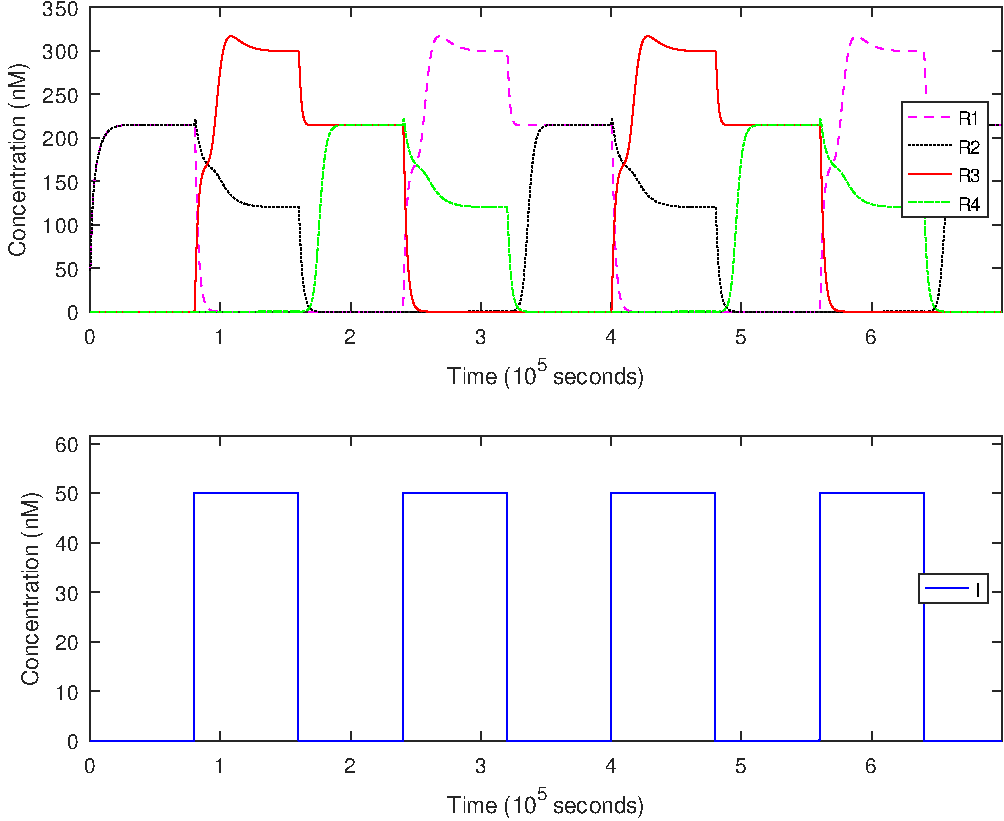
\includegraphics[width=\textwidth]{freqdiv-square}
      \caption{@FIXME.}
      \label{fig.freqdiv-square}
    \end{figure}

    \begin{figure}[!htbp]
      \centering
      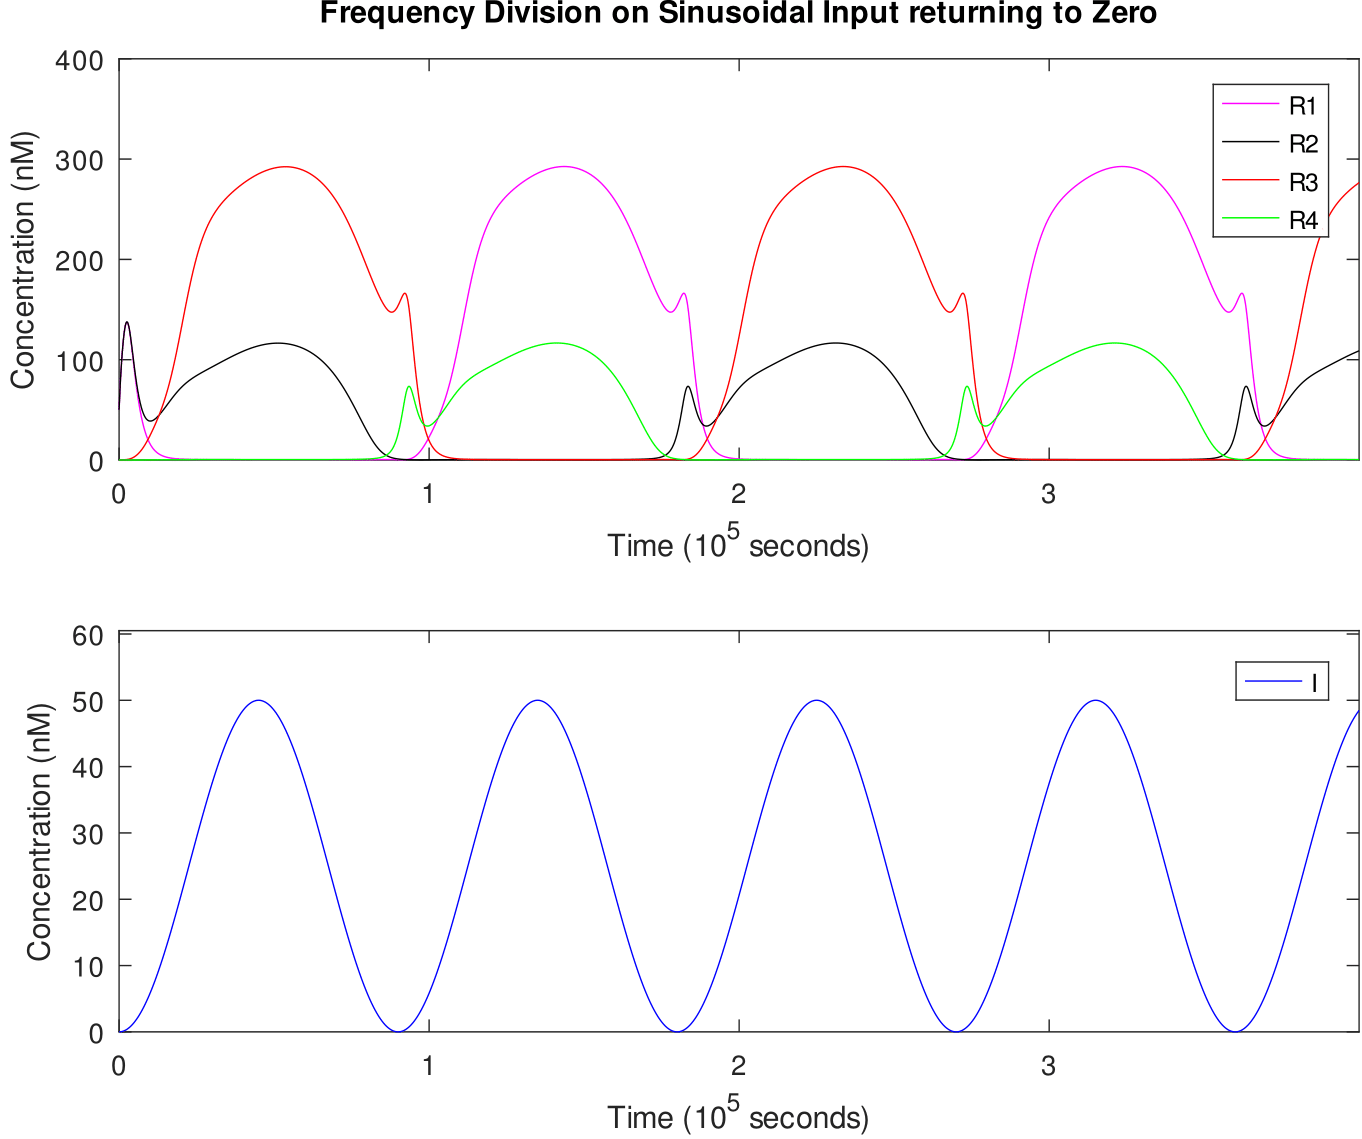
\includegraphics[width=\textwidth]{freqdiv-zero}
      \caption{@FIXME.}
      \label{fig.freqdiv-zero}
    \end{figure}

    \begin{figure}[!htbp]
      \centering
      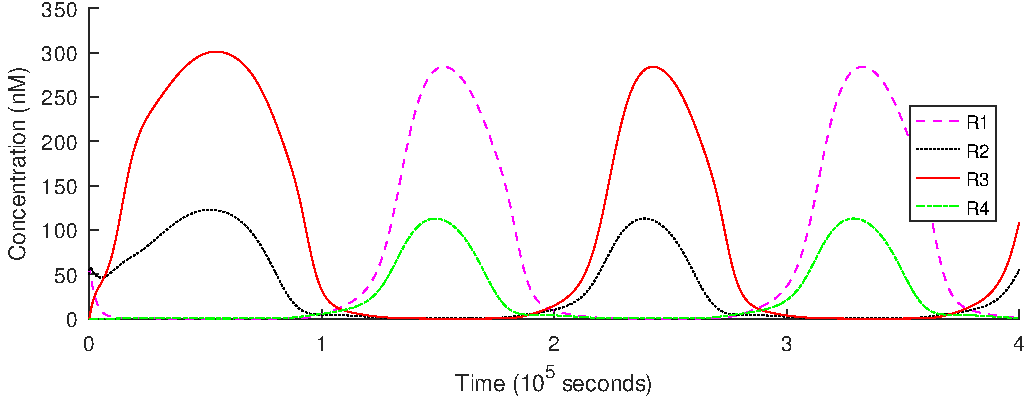
\includegraphics[width=\textwidth]{freqdiv-qssa}
      \caption{@FIXME.}
      \label{fig.freqdiv-qssa}
    \end{figure}

    \begin{figure}[!htbp]
      \centering
      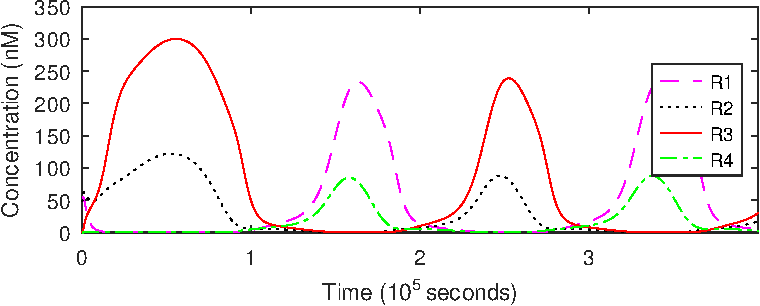
\includegraphics[width=\textwidth]{freqdiv-full}
      \caption{@FIXME.}
      \label{fig.freqdiv-full}
    \end{figure}

    Notice that with a sinusoidal input, the output signals from the \ac{qssa} model have constant amplitude, whereas in the full model the first concentration peak of proteins R2 and R3 are higher than the following ones.
    This suggests \acs{mrna} reactions stabilize quicker in the first $10^5$ seconds and thus the approximation is more accurate at those instants.
    After that moment, however, the reduced model exhibits a persistent error in relation to the complete one, which can be observed by comparing concentration levels reached during oscillation peaks in Figures \ref{fig.freqdiv-qssa} and \ref{fig.freqdiv-full}.

    In those simulations, while R1 and R4 concentrations in the full model reach \textit{maxima} valued at \SI{238.29}{\nano M} and \SI{87.62}{\nano M} respectively, the reduced model (again, this is the one presented in the original paper) goes up to \SI{283.96}{\nano M} and \SI{113.05}{\nano M} for each of these proteins.
    Peak values of R3 follow R1 closely and the same happens with R2 and R4.
    This offset distinguishing the two models happens because the \ac{qssa} used to derive the reduced \ac{ode} system considers a separation of time-scales between reactions which regulate \acs{mrna} production and those which describe protein translation.
    In the approximation, the former reactions are assumed to reach equilibrium instantaneously relative to the latter.
    Thus, the difference is a consequence of the fact that the original model maintains itself in a dynamic state that never actually reaches equilibrium, as it perpetually oscillates \cite{ingalls}.


  \subsection{Bifurcation Analysis}

    As in the original work, we observe different behaviours can be obtained by holding input concentration constant at certain ranges.
    More importantly, it is how \citet{originals} discovered the model's multiple extra functionalities.
    The six experiments in the bifurcation analysis were reproduced, where input levels are the same as given and initial conditions used are $R1=R2=0nM$ and $R3=R4=50nM$ for simulations $1b$ and $4c_{2}$ and $R1=R2=50nM$ and $R3=R4=0nM$ for all others.
    The original text states simulations labeled $4c_{1}$ and $1b$ use the same initial conditions as $4c_{2}$ and $1a$ respectively.
    We believe these were typographical errors, as such settings would lead the mentioned experiments to be exactly the same under deterministic semantics and this is not what is exhibited.

    \begin{figure}[!htbp]
      \centering
      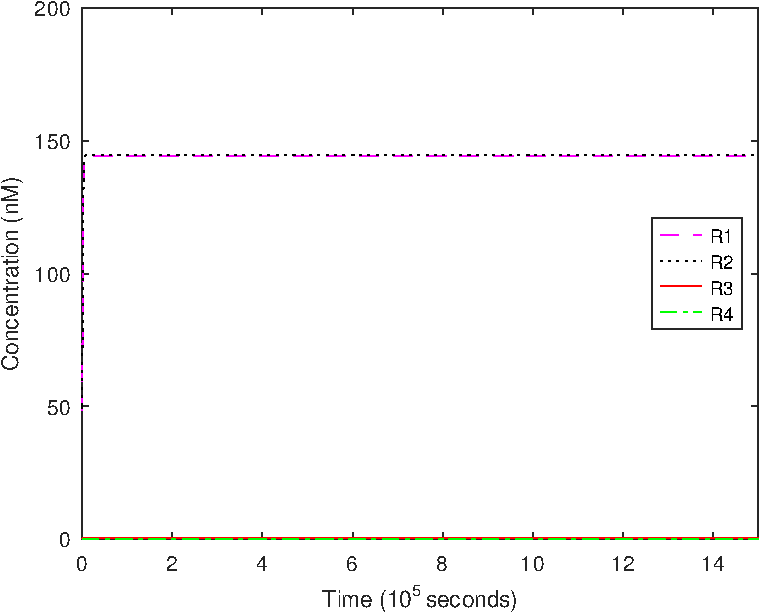
\includegraphics[width=\textwidth]{bifurcation-1a}
      \caption{@FIXME.}
      \label{fig.bifurcation-1a}
    \end{figure}

    \begin{figure}[!htbp]
      \centering
      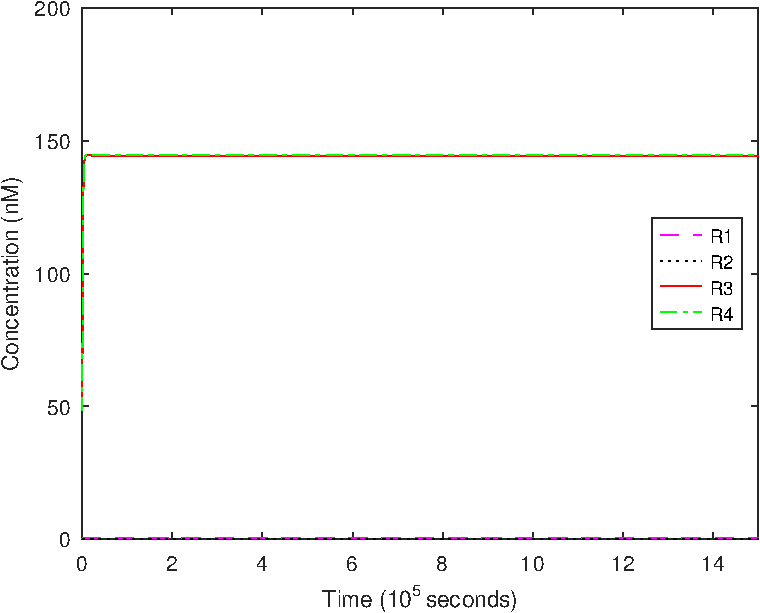
\includegraphics[width=\textwidth]{bifurcation-1b}
      \caption{@FIXME.}
      \label{fig.bifurcation-1b}
    \end{figure}

    \begin{figure}[!htbp]
      \centering
      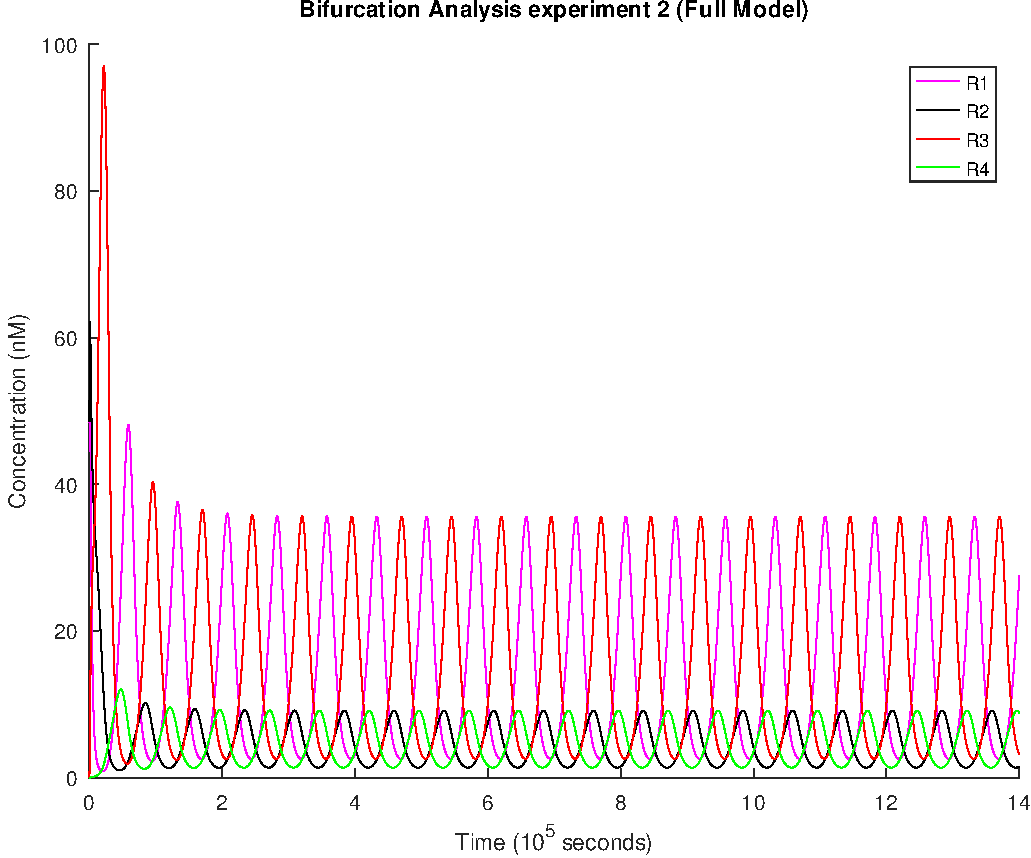
\includegraphics[width=\textwidth]{bifurcation-2-full}
      \caption{@FIXME.}
      \label{fig.bifurcation-2-full}
    \end{figure}

    \begin{figure}[!htbp]
      \centering
      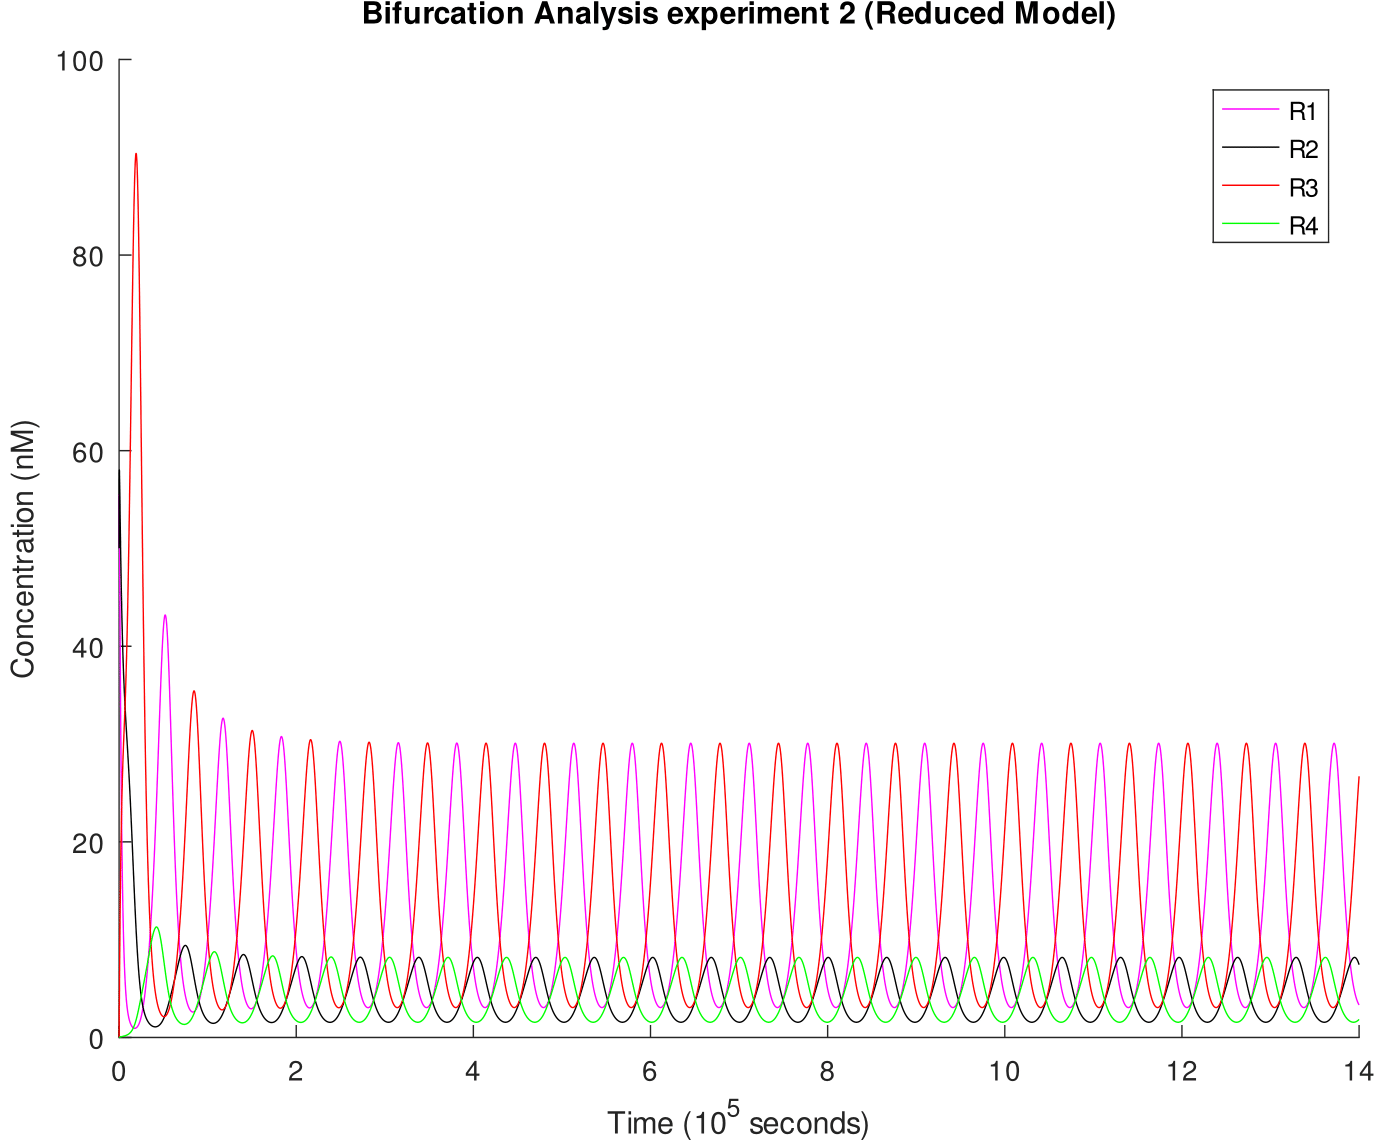
\includegraphics[width=\textwidth]{bifurcation-2-qssa}
      \caption{@FIXME.}
      \label{fig.bifurcation-2-qssa}
    \end{figure}

    \begin{figure}[!htbp]
      \centering
      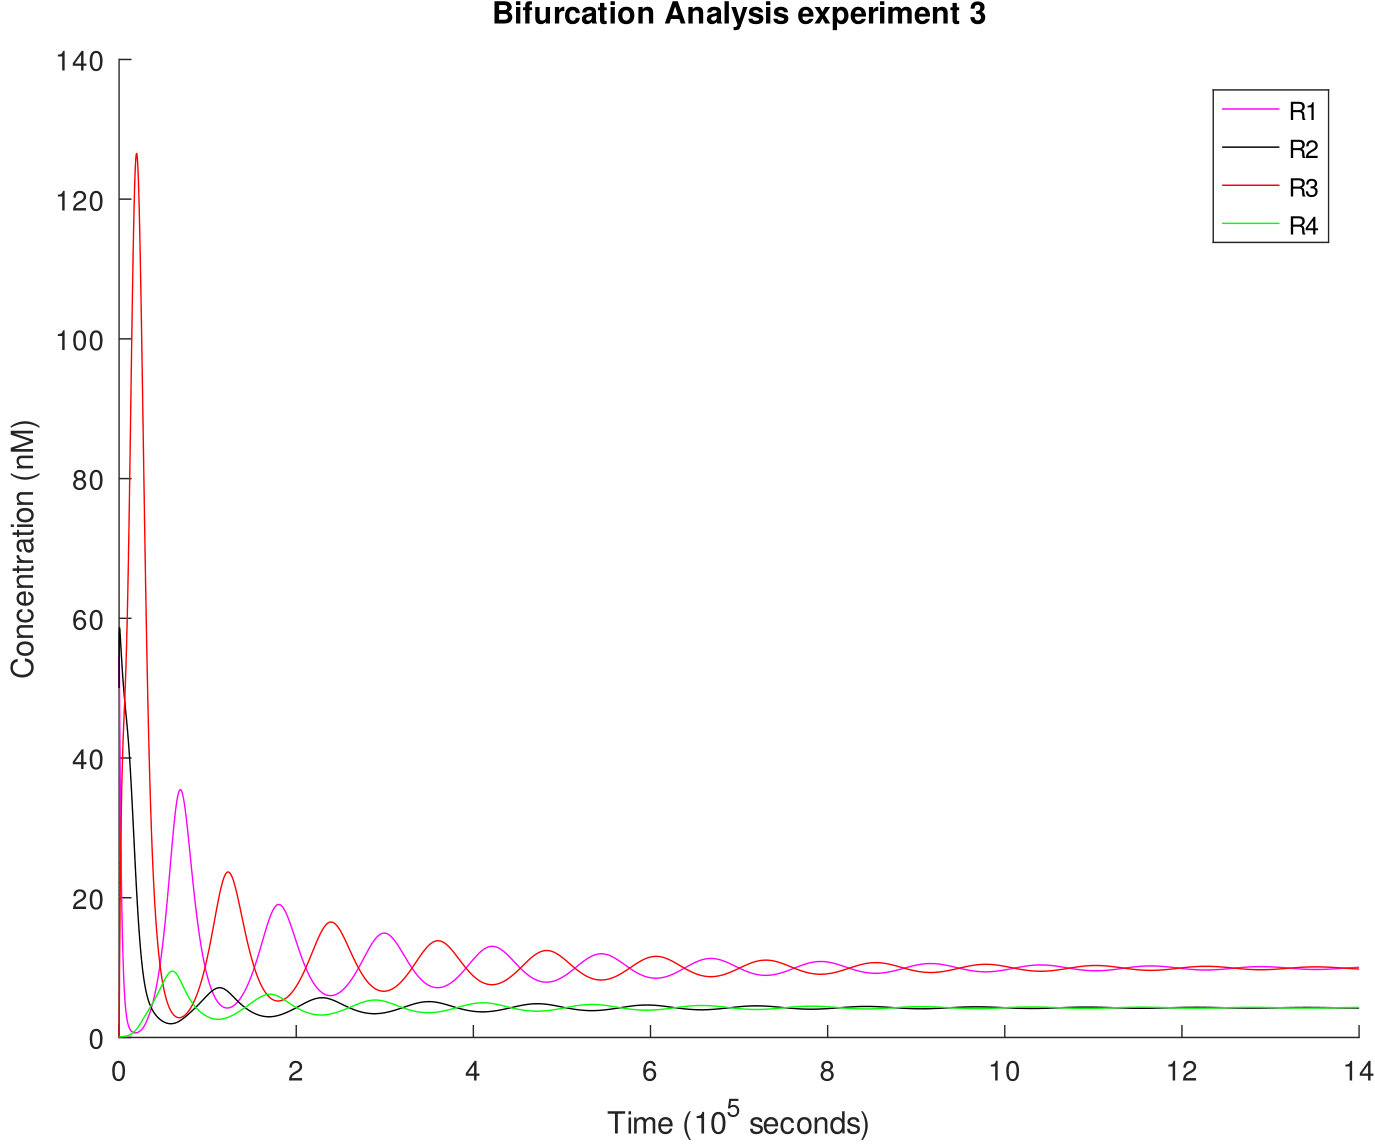
\includegraphics[width=\textwidth]{bifurcation-3}
      \caption{@FIXME.}
      \label{fig.bifurcation-3}
    \end{figure}

    \begin{figure}[!htbp]
      \centering
      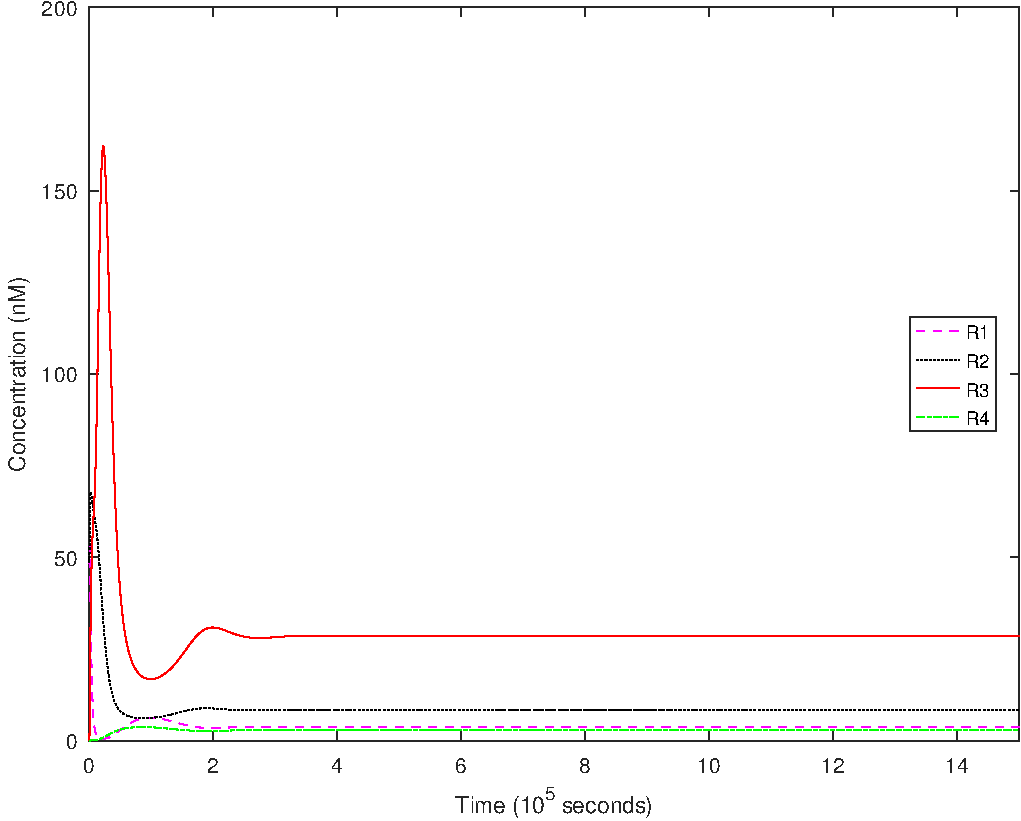
\includegraphics[width=\textwidth]{bifurcation-4c1}
      \caption{@FIXME.}
      \label{fig.bifurcation-4c1}
    \end{figure}

    \begin{figure}[!htbp]
      \centering
      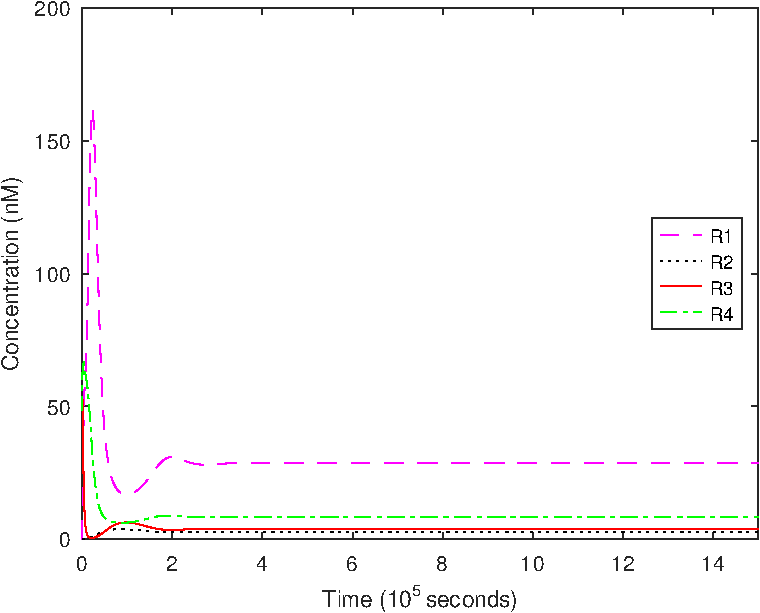
\includegraphics[width=\textwidth]{bifurcation-4c2}
      \caption{@FIXME.}
      \label{fig.bifurcation-4c2}
    \end{figure}

    Once again, oscillation amplitude differs between models, with R1 and R4 each peaking at \SI{35.60}{\nano M} and \SI{9.16}{\nano M} in the complete system (Figure \ref{fig.bifurcation-2-full}) while going up to \SI{30.08}{\nano M} and \SI{8.18}{\nano M} in the \ac{qssa} reduction (Figure \ref{fig.bifurcation-2-qssa}).
    Other experiments do not present such significant offset.


  \subsection{Self-induced Oscillator}

    @TODO


  \subsection{Toggle Switch}

    As revealed during bifurcation analysis, the network exhibits bistability when input concentration is held constant outside the oscillatory range.
    Figures \ref{fig.switch-A} to \ref{fig.switch-D} illustrate simulations with the system being used as a toggle switch which is "triggered" by varying binding affinity of particular repressors.
    These experiments were exactly reproduced from the reference work without any difficulties, as all parameters are given, and no significant difference is found between reduced and full models.

    \begin{figure}[!htbp]
      \centering
      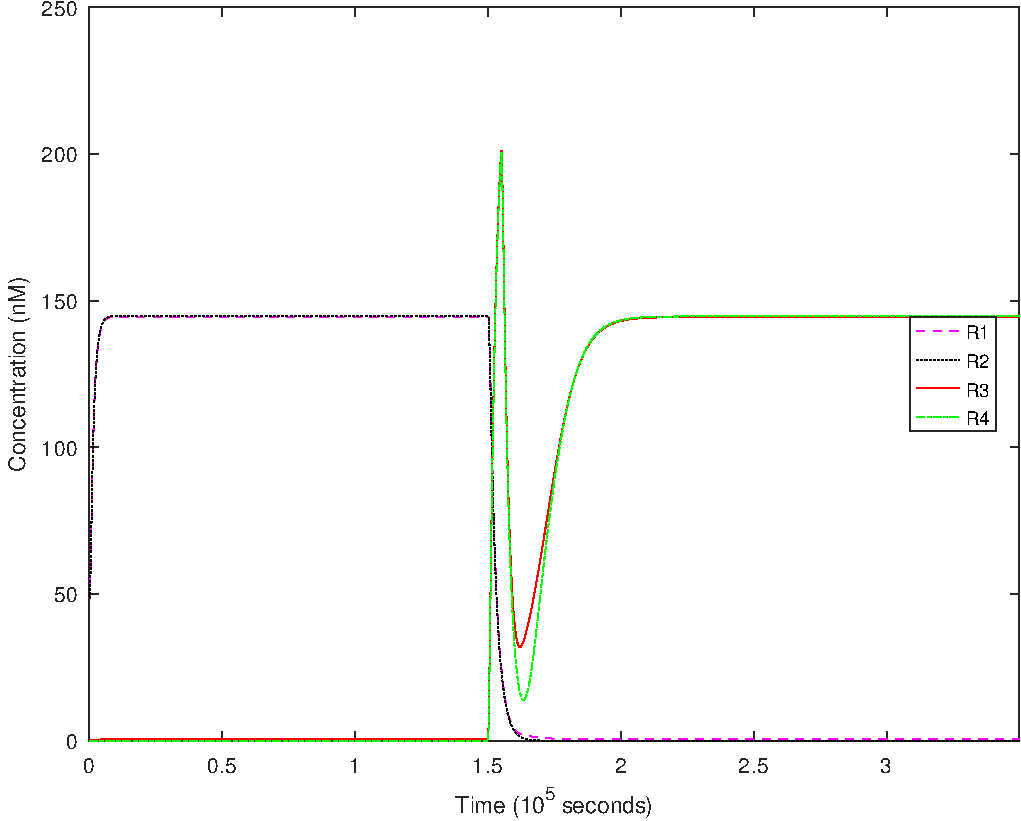
\includegraphics[width=\textwidth]{switch-A}
      \caption{@FIXME.}
      \label{fig.switch-A}
    \end{figure}

    \begin{figure}[!htbp]
      \centering
      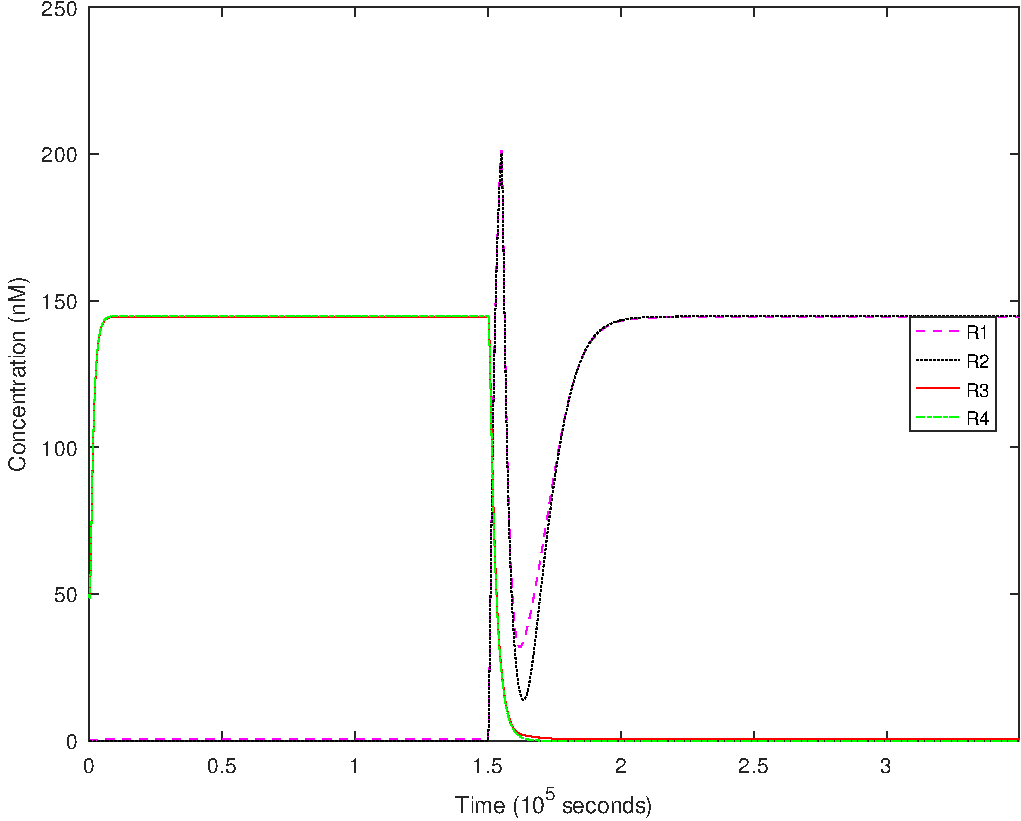
\includegraphics[width=\textwidth]{switch-B}
      \caption{@FIXME.}
      \label{fig.switch-B}
    \end{figure}

    \begin{figure}[!htbp]
      \centering
      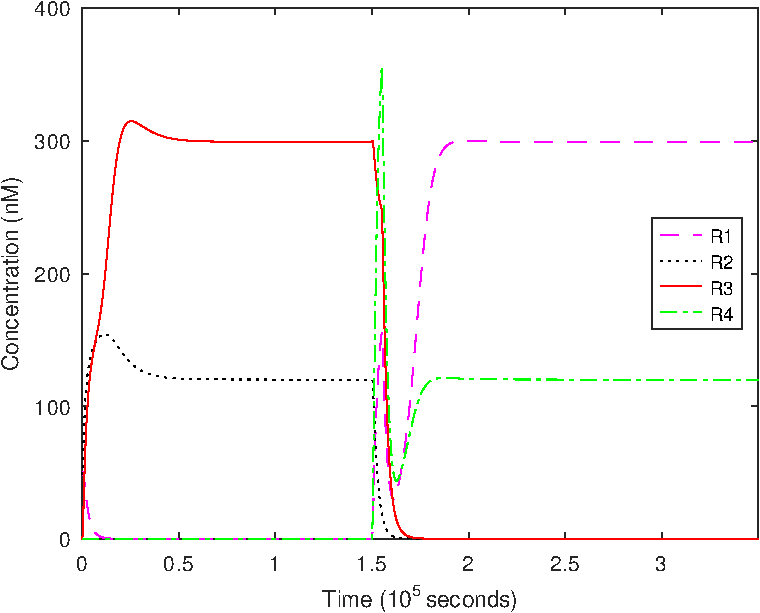
\includegraphics[width=\textwidth]{switch-C}
      \caption{@FIXME.}
      \label{fig.switch-C}
    \end{figure}

    \begin{figure}[!htbp]
      \centering
      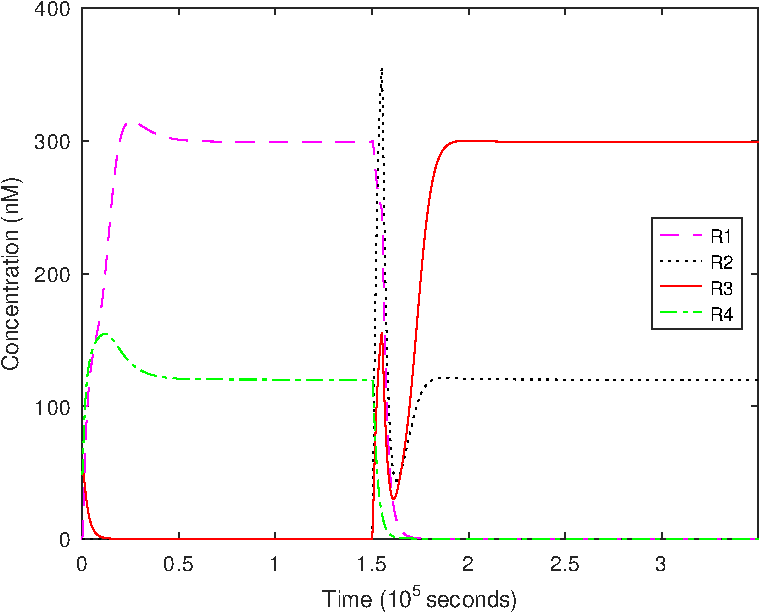
\includegraphics[width=\textwidth]{switch-D}
      \caption{@FIXME.}
      \label{fig.switch-D}
    \end{figure}


  \subsection{Stochastic Simulations}

    % # 1/14
    % seed=2.832228911341789e-220 # 3 red
    % seed=1.093374056741564e-12  # normal
    % seed=3.079242033197292e-283 # 2 magenta, negative
    % seed=4.644825783344441e+132 # 2 red, 3 magente, negative


  \subsection{Leaky Promoter Experiments}

    ...


\section{Conclusion}

  % We highlight the idea that as synthetic networks grow in complexity and size, multi-functionality may arise more frequently and become difficult to avoid.
  % While this can bring the benefits of reusable programmable components, it might also end up becoming a nuisance if models start behaving unexpectedly under the influence of certain inputs.

  \textit{Relembrar objetivos.
  Explicar como foi (ou não) possível replicar o artigo original, destacando quaisquer diferenças nos trabalhos.
  Apresentar trabalhos futuros.}
